\documentclass[11pt,a4paper]{article}
\usepackage[a4paper,margin=2.15cm]{geometry}
\usepackage{setspace}
\usepackage{graphicx}
\usepackage{booktabs}
\onehalfspacing
\setlength{\parskip}{0.15em}
\setlength{\parindent}{1.05em}
\pdfinfoomitdate=1
\begin{document}

\begin{titlepage}
\centering
\vspace*{22mm}
{\Large Visitor mix and hotel occupancy by star class in Macao\par}
\vspace{0.8em}
{\large Phase A draft\par}
\vspace{0.8em}
CS482 Data Science\par
Group X\par
\vspace{0.6em}
21 November 2026\par
\vspace{1.6em}
\begin{minipage}{\textwidth}
\raggedright
Draft for the Phase A checkpoint. The cover, references, contribution statement, and AI declaration are outside the main-text page count. Every number in the main text is copied from the Phase A output files. A deep-learning extension is specified in the project plan and is not part of this draft.
\end{minipage}
\end{titlepage}

\section{Introduction}
The question is whether the conditional association between Macao's visitor mix and hotel occupancy differs by star class after the pandemic, and whether next month's occupancy can be forecast from information dated no later than the current month. The outcome is the monthly occupancy rate of guest rooms, in percent, for the four star classes DSEC publishes: 5-star, 4-star, 3-star, and 2-star. The window is 2010-01 to 2026-09.

Three hypotheses were fixed before any model was fit. H1 says that, after the pandemic, the association between log overnight visitors and occupancy differs between 5-star and 3-star hotels. The null is that the two post-pandemic slopes are equal. H2 says that the association between the same-day visitor share and occupancy differs between the post-pandemic and the pre-pandemic period. The null is that the change in that slope is zero. H3 says that a global LightGBM, using only lags and the known calendar, forecasts next month's occupancy more accurately than a seasonal naive forecast and than a per-class SARIMAX. The decision rule was fixed in advance: H3 is supported only if LightGBM has the lower pooled test mean absolute error against both baselines and both pooled Holm-adjusted \(p\)-values are below 0.05.

Hotel operators and the tourism authority can use the description to see which associations the published series actually show. The results are descriptive, associational, and predictive. They are not causal estimates, and they are not a pricing or staffing rule.

\section{Data Collection and Preparation}
Visitor arrivals and hotel series are taken from the DSEC Time Series Database behind the visitor page (\texttt{dsec.gov.mo/en-US/Statistic?id=402}) and the package-tour and hotel page (\texttt{id=403}). The snapshot was checked against DSEC's latest monthly workbooks. Mainland public holidays come from the State Council notices on gov.cn for 2010--2026, including three later notices that changed a published schedule. Typhoon days come from the Macao Meteorological and Geophysical Bureau: a day counts if tropical cyclone signal No.~8 or higher was in force for any part of that calendar day. Gaming revenue is optional in the plan and is not used.

The frozen panel has 804 rows: 4 star classes by 201 months, from 2010-01 to 2026-09, with no missing value. The plan's periods are 120 pre-pandemic months (2010-01 to 2019-12), January 2020 as a transition month, 35 pandemic months (2020-02 to 2022-12), and 45 post-pandemic months (2023-01 to 2026-09). The main sample is the pre-pandemic and post-pandemic months: 165 months and 660 rows, of which 180 are post-pandemic. Occupancy in the window runs from 5.0 to 97.2 percent. The window contains 115 holiday periods (492 holiday days) and 44 typhoon days.

DSEC's four labels are present in every month. The hotels inside a label are not a fixed set: the establishment count of a class changes in 87 tier-months, and rooms change by 10 percent or more in 22 tier-months. The largest jump is 3-star rooms in 2016-09, from 2,528 to 5,477. Shares are computed from the published counts. The international share is 100 times one minus the share of arrivals whose travel document was issued in the mainland, Hong Kong, or Taiwan. Holiday days are stored twice: the final schedule, used in the ex-post regression, and the schedule published by the end of the previous month, used as the forecast feature. Those two counts differ in four months, and in none of the test targets.

The forecast split was frozen with the panel. There are 36 validation origins, all before the first test origin, and 26 test origins from 2024-07 to 2026-08 (104 forecasts, one month ahead). The first month with all twelve lags is 2011-01. The forecast of month \(t+1\) uses DSEC values up to month \(t\) as published on the download date. DSEC's publication lag and later revisions are not reproduced, so the errors are not those of a forecast made in real time. The frozen panel hash begins 9c9547d653c5.

\section{Methods}
The exploratory description is separate from the tests. Occupancy is decomposed with a robust STL of period 12, one fit per star class in the pre-pandemic block and one in the post-pandemic block, with a seasonal pattern that is constant inside the block. The pandemic months are not decomposed: one fit across them pushed the collapse into the seasonal component of the months after them. Change points in the three visitor-mix shares are estimated with PELT on the seasonally adjusted series, for a piecewise-constant mean, with segments of at least 12 months. The penalty is \(2 \times \mathrm{noise\_sd}^{2} \times \ln n\), and the same run is reported at half, twice, and four times that penalty. The period boundaries used below are the ones in the plan. They were not taken from PELT.

The ex-post model, fit by least squares on the main sample, is
\[
O_{i,t} = a_i + a^{\mathrm{post}}_i \mathrm{post}_t + \mathrm{month}_t + (b_i + b^{\mathrm{post}}_i \mathrm{post}_t)\log V_t + (c + c^{\mathrm{post}}\mathrm{post}_t) S_t + \mathrm{controls} + e_{i,t}.
\]
\(O\) is occupancy in percent, \(\log V\) is log overnight visitors, and \(S\) is the same-day share in percent. The controls, each with one coefficient, are the international share, the package-tour share, log rooms, holiday days, and typhoon days. Standard errors are Driscoll--Kraay with a Bartlett kernel. The bandwidth is \(\lfloor 4(T/100)^{2/9}\rfloor\), which is 4 for \(T=165\), and lags are counted in calendar months, so nothing is carried across the gap between December 2019 and January 2023. Tests are two-sided at 0.05 with a normal reference and a 95 percent interval. H1 and H2 are adjusted by Holm over those two tests. Two secondary Wald tests are reported and are not part of that family: equality of the four post-pandemic slopes, and a Chow-type test of the five post interactions on the two focal regressors. Five sensitivity runs were specified in advance. Ljung--Box statistics and a Breusch--Pagan statistic are reported and do not change the model, the standard errors, or the tests.

The forecast uses three models, each refit at every origin on target months up to that origin. The seasonal naive forecast is occupancy in the same month one year earlier. SARIMAX is fit per star class, with the holiday counts known at the origin as exogenous terms; occupancy from 2020-01 to 2022-12 is treated as missing in the main run. LightGBM is one global model. Its features are the star class, four calendar variables of the target month, and lags of 1, 2, 3, and 12 months. No other variable dated in the target month is used, and typhoon days of the target month are never a feature. Orders and the LightGBM grid point are chosen by validation mean absolute error. The candidates differ in differencing, so AIC and BIC are not used. The test origins are then forecast once. Accuracy is MAE, RMSE, and MASE, in percentage points, per class and pooled. Comparisons use the Diebold--Mariano test with the Harvey--Leybourne--Newbold correction, absolute-error loss, and horizon 1, Holm-adjusted over the ten tests (two baselines by four classes and the pooled series). TreeSHAP values, path-dependent, are computed for the LightGBM fit at each test origin. The background is that origin's training window, the output is the forecast in percentage points, and the values are checked for additivity.

\section{Results}
Mean monthly visitor mix moves from the pre-pandemic period to the post-pandemic period as follows. The same-day share goes from 51.35 to 55.34 percent, the international share from 9.82 to 6.26, and the package-tour share from 28.05 to 5.36. Mean overnight arrivals go from 1,263,786 to 1,315,841 a month. In the pandemic months the international share averages 0.5 percent and the package-tour share 0.5 percent. Change points that remain at every reported penalty are 2021-08 and 2022-08 for the same-day share; 2020-03 for the international share; 2020-01 and 2023-03 for the package-tour share. Mean occupancy goes from 85.6 to 89.0 percent for 5-star hotels, 86.9 to 83.0 for 4-star, 85.6 to 83.6 for 3-star, and 73.7 to 88.0 for 2-star. After the pandemic the seasonal peak of occupancy is August in all four classes. These descriptions are not tests of H1--H3.

On the main sample of 660 rows, the regression has 34 coefficients and \(R^{2}=0.755\). The H1 contrast, 5-star minus 3-star in the post-pandemic slope on log overnight visitors, is 18.33 (SE 6.94, 95 percent CI 4.73 to 31.93, Holm-adjusted \(p=0.016\)). The null is rejected at 0.05. The post-pandemic slope itself is 21.23 for 5-star hotels (CI 14.28 to 28.17) and 2.89 for 3-star hotels (CI -8.83 to 14.62). A month with 10 percent more overnight visitors, the other regressors equal, has about 2.02 points higher 5-star occupancy and about 0.28 points higher 3-star occupancy. The H2 change in the same-day-share slope is 0.04 (SE 0.15, CI -0.26 to 0.34, Holm-adjusted \(p=0.804\)). The null is not rejected. That is not evidence that the change is zero: the interval runs from -0.26 to 0.34 points of occupancy per point of same-day share. The secondary tests reject equal post-pandemic slopes (\(\chi^{2}(3)=15.3\), \(p=0.002\)) and reject the five post interactions jointly (\(\chi^{2}(5)=36.4\), \(p=< 0.001\)).

The same sign for H1 appears in all seven runs, and the null is rejected after Holm in six. In the fully interacted run the Holm-adjusted \(p\) is 0.060. H2 is rejected after Holm in one run only, the run with class-specific trends (estimate 0.39, Holm-adjusted \(p=0.020\)). The H2 result depends on how the trend is modelled. The confirmatory result remains the main run. Ljung--Box \(p\)-values are below 0.05 in 14 of 16 class-block-lag cells, and the Breusch--Pagan \(p\) is < 0.001. The residuals are serially correlated and heteroskedastic. The model was not changed on that basis.

Pooled test MAE is 2.06 for LightGBM, 2.36 for SARIMAX, and 3.26 for the seasonal naive forecast (RMSE 2.83, 3.42, 4.11; MASE 0.47, 0.53, 0.75). LightGBM is lower than both baselines. Against the seasonal naive forecast the pooled loss difference is -1.19 (CI -1.92 to -0.46, Holm-adjusted \(p=0.022\)). Against SARIMAX it is -0.30 (CI -1.04 to 0.44, Holm-adjusted \(p=1.000\)). Only the first of those two is below 0.05, so H3 is not supported. Per class, LightGBM MAE is 1.66, 2.16, 2.45, and 1.99. No class-level comparison with SARIMAX has a Holm-adjusted \(p\) below 0.05. On the logit scale, with metrics back-transformed to percentage points, pooled MAE is 1.98 and 2.25, and H3 is again not supported. Keeping the pandemic months in training raises LightGBM's pooled MAE to 4.52, above SARIMAX at 2.85 and the seasonal naive forecast at 3.26; those LightGBM forecasts sit -3.00 points below the observed occupancy on average.

The chosen main-run SARIMAX order is (1, 0, 1) with seasonal order (0, 1, 1, 12) for 5-star hotels, and (1, 1, 1) with seasonal order (0, 1, 1, 12) for the other three classes. The chosen LightGBM point is 8 leaves, at least 10 rows per leaf, and 400 trees. No validation candidate failed to converge, and all 312 test fits converged. TreeSHAP, which describes this model and not a causal contribution, puts the largest mean absolute value on occupancy one month earlier (1.82 points), then on overnight visitors one year earlier (1.23), then on guest rooms one month earlier (1.22). The largest gap between the forecast and the base value plus the SHAP values is under \(10^{-12}\).

\begin{center}
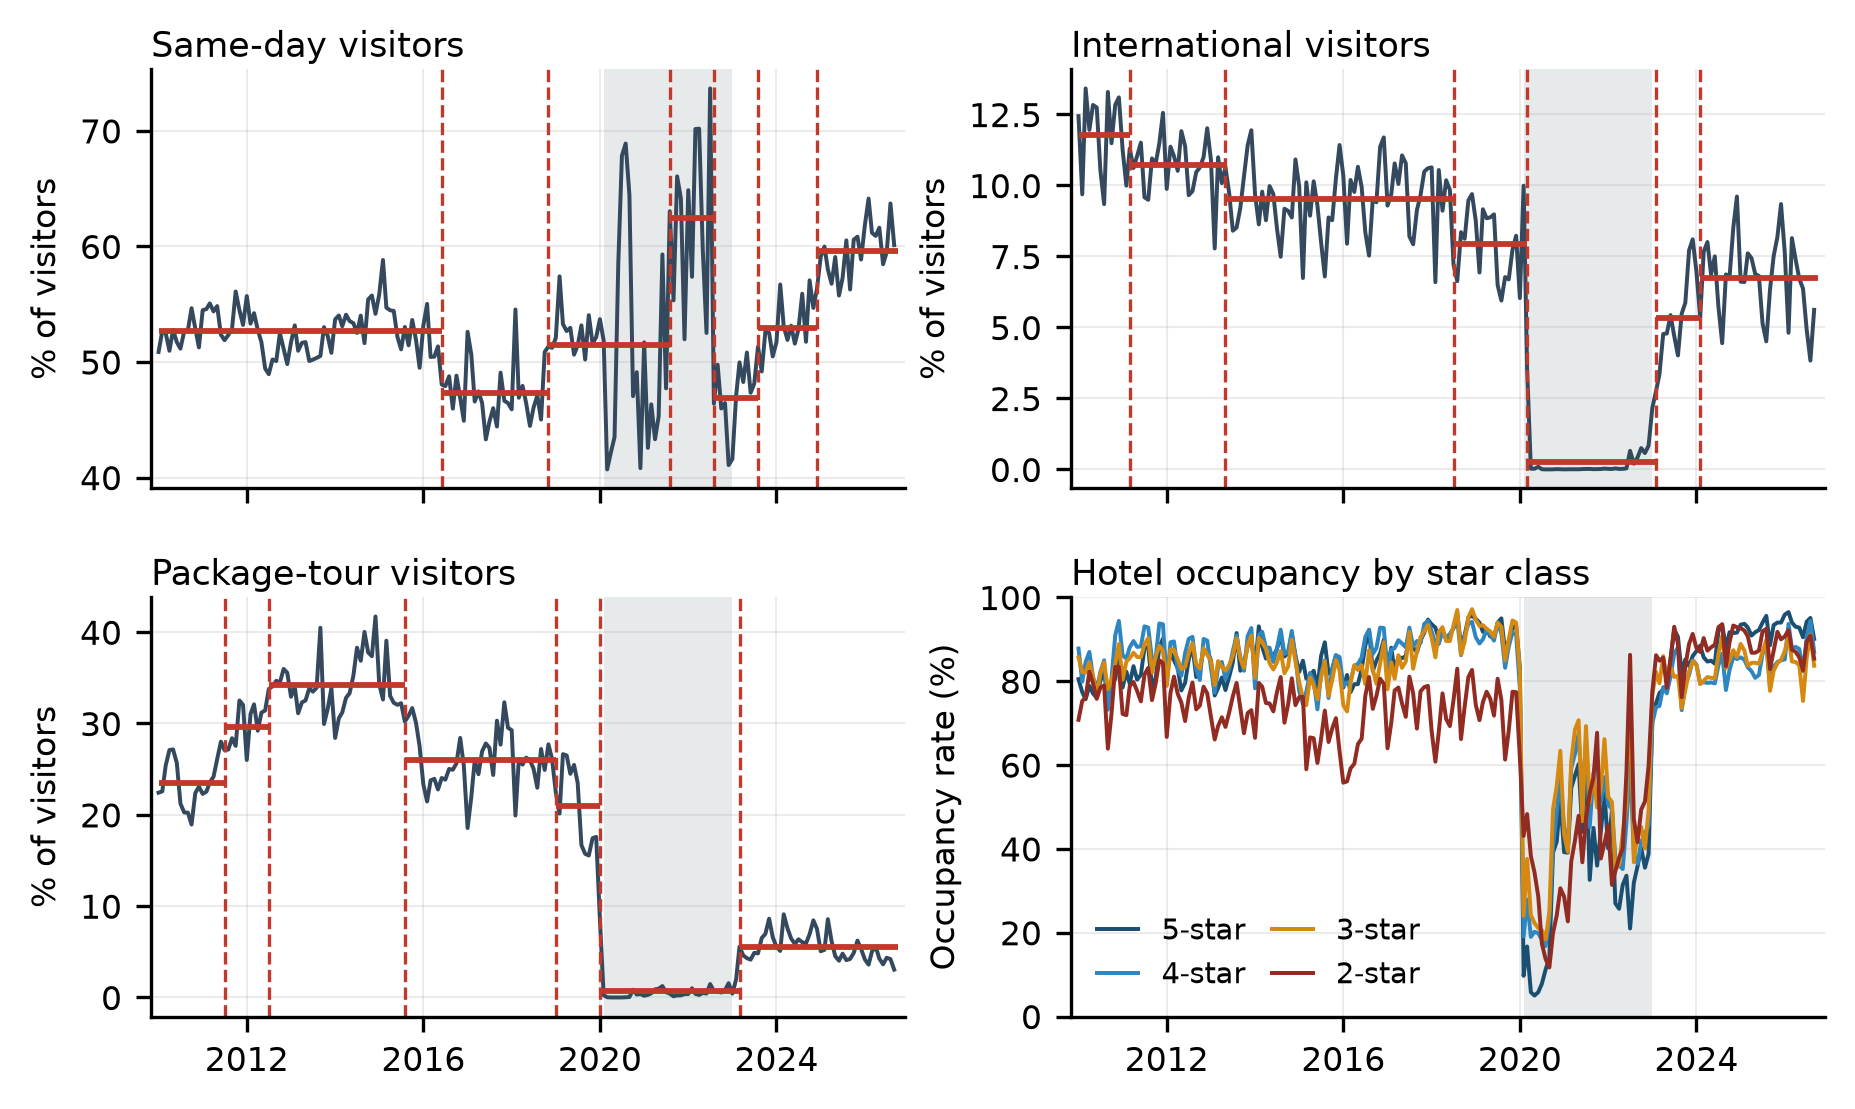
\includegraphics[width=\textwidth,height=0.26\textheight,keepaspectratio]{../outputs/figures/fig1_visitor_mix_and_occupancy.png}\\[2pt]
{\small Figure 1. Visitor-mix shares with PELT change points, and occupancy by star class. The grey band is the plan's pandemic window. The marks are exploratory.}
\end{center}

\begin{center}
{\small
\begin{tabular}{lrrrr}
\toprule
Quantity & Estimate & SE & 95\% CI & Holm \(p\) \\
\midrule
H1, post slope, 5-star minus 3-star & 18.33 & 6.94 & 4.73 to 31.93 & 0.016 \\
H2, change in the same-day slope & 0.04 & 0.15 & -0.26 to 0.34 & 0.804 \\
5-star post slope on log overnight visitors & 21.23 &  & 14.28 to 28.17 &  \\
3-star post slope on log overnight visitors & 2.89 &  & -8.83 to 14.62 &  \\
\midrule
Model (pooled test) & MAE & RMSE & MASE & \\
\midrule
LightGBM & 2.06 & 2.83 & 0.47 &  \\
SARIMAX & 2.36 & 3.42 & 0.53 &  \\
Seasonal naive & 3.26 & 4.11 & 0.75 &  \\
\bottomrule
\end{tabular}
}\\[2pt]
{\small Table 1. Confirmatory contrasts, in points of occupancy, and pooled test accuracy. H1 and H2 use Driscoll--Kraay standard errors and Holm adjustment over the two tests. MAE, RMSE, and MASE are in percentage points. The forecast rows are not a causal comparison.}
\end{center}

\begin{center}
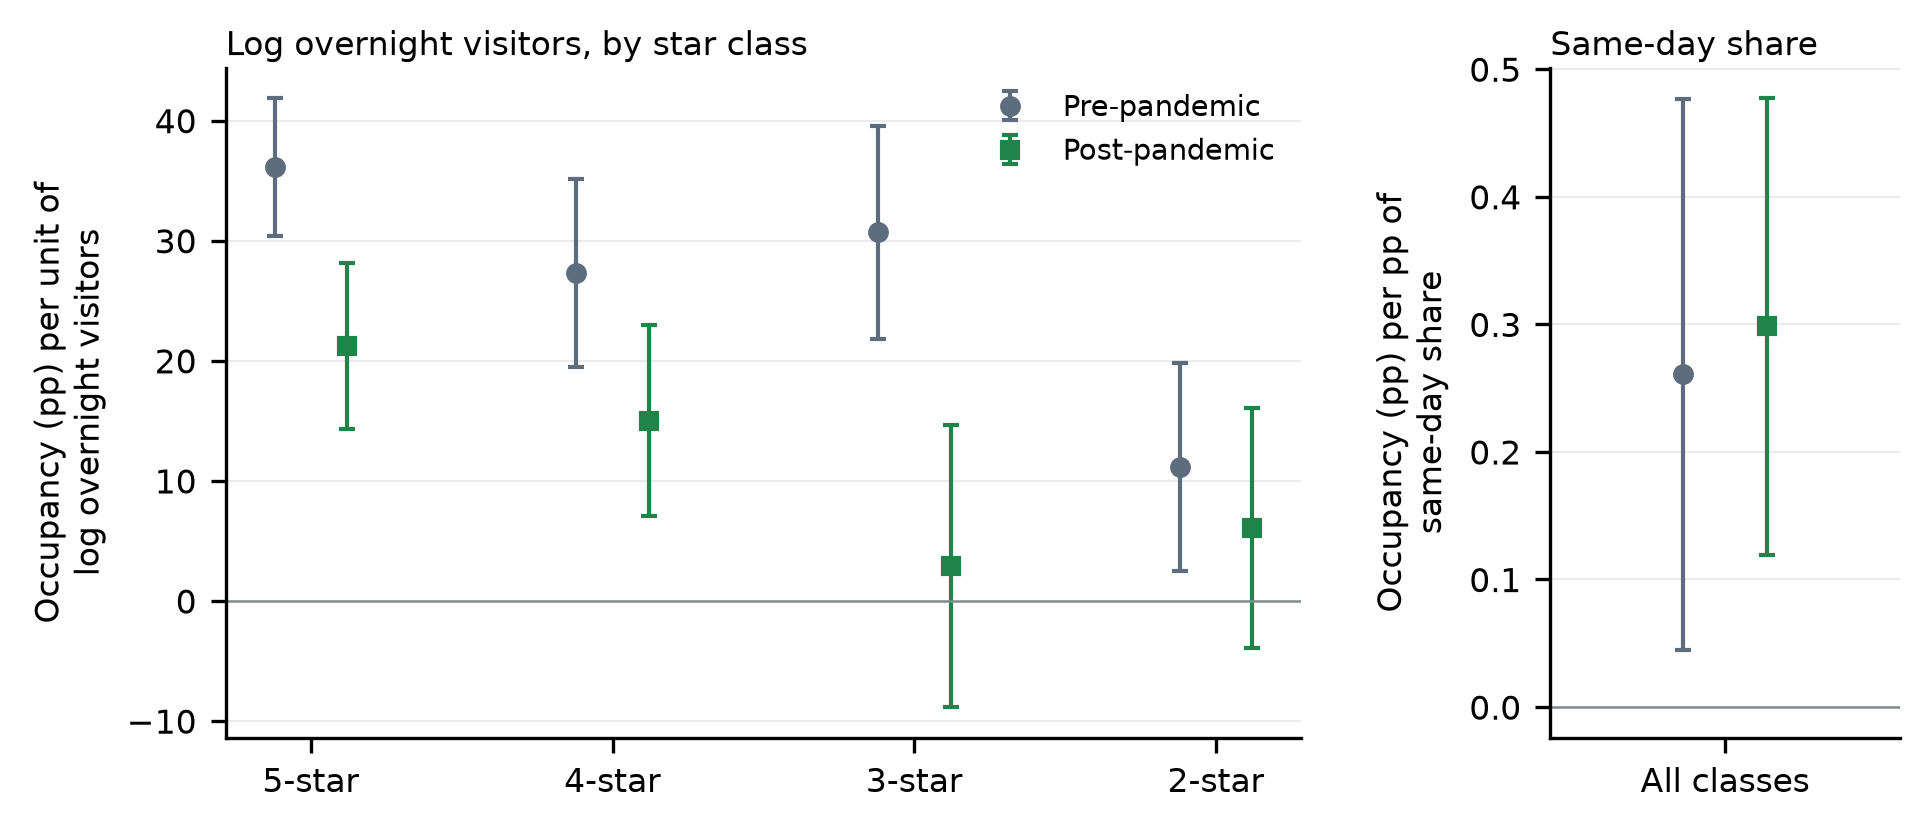
\includegraphics[width=0.92\textwidth,height=0.16\textheight,keepaspectratio]{../outputs/figures/fig_regression_slopes_by_class.png}\\[2pt]
{\small Figure 2. Conditional slopes before and after the pandemic, with 95 percent intervals. A slope is an association in the regression, not a causal quantity.}
\end{center}

\section{Discussion}
H1 is supported in the pre-specified model: after the pandemic, occupancy moves with overnight visitors more strongly for 5-star hotels than for 3-star hotels, by 18.33 points of occupancy per unit of log overnight visitors (CI 4.73 to 31.93). H2 is not supported. The data are compatible with a change in the same-day slope anywhere from -0.26 to 0.34, and a different trend specification rejects the null, so the result should be read with that sensitivity next to it. H3 is not supported. LightGBM beats the seasonal naive forecast on the pooled test series and does not beat SARIMAX by a margin the ten-test correction can separate from zero. The pooled difference against SARIMAX is -0.30 points, and the interval crosses zero.

Two uses follow, both short of a recommendation to change a policy. A hotel that still applies the pre-pandemic slope of overnight visitors to a 3-star occupancy plan is using a stronger association than the post-pandemic sample shows. A forecast user who adopts LightGBM instead of SARIMAX sees a pooled MAE difference of -0.30 points in this window, LightGBM minus SARIMAX, and that difference is not distinguishable from zero at the pre-specified threshold. Neither statement is a causal claim about marketing, pricing, or the border regime.

The limits are the ones the design cannot remove. The post-pandemic block has only 45 months, so several intervals are wide, and the normal reference rests on 165 months of serially correlated residuals. A star class is not a fixed set of hotels: establishment counts change, and the rise in 2-star mean occupancy from 73.7 to 88.0 sits next to that recomposition. DSEC revises its series, and the backtest does not replay those revisions. The regression uses same-month visitor counts, so it describes the month after the fact and shares the seasonal pattern of the two series. Putting the pandemic months into the training window makes the LightGBM forecasts worse, which is a reason to keep the pre-specified exclusion rather than a reason to search for a better one after the fact. Phase B, the deep-learning extension, is not estimated here.

\clearpage
\begin{thebibliography}{9}
\bibitem{cleveland1990} Cleveland, R.~B., Cleveland, W.~S., McRae, J.~E., and Terpenning, I. (1990). STL: A seasonal-trend decomposition procedure based on loess. \textit{Journal of Official Statistics}, 6(1), 3--73.
\bibitem{diebold1995} Diebold, F.~X., and Mariano, R.~S. (1995). Comparing predictive accuracy. \textit{Journal of Business and Economic Statistics}, 13(3), 253--263.
\bibitem{driscoll1998} Driscoll, J.~C., and Kraay, A.~C. (1998). Consistent covariance matrix estimation with spatially dependent panel data. \textit{Review of Economics and Statistics}, 80(4), 549--560.
\bibitem{harvey1997} Harvey, D., Leybourne, S., and Newbold, P. (1997). Testing the equality of prediction mean squared errors. \textit{International Journal of Forecasting}, 13(2), 281--291.
\bibitem{holm1979} Holm, S. (1979). A simple sequentially rejective multiple test procedure. \textit{Scandinavian Journal of Statistics}, 6(2), 65--70.
\bibitem{killick2012} Killick, R., Fearnhead, P., and Eckley, I.~A. (2012). Optimal detection of changepoints with a linear computational cost. \textit{Journal of the American Statistical Association}, 107(500), 1590--1598.
\bibitem{lundberg2017} Lundberg, S.~M., and Lee, S.-I. (2017). A unified approach to interpreting model predictions. \textit{Advances in Neural Information Processing Systems}, 30.
\end{thebibliography}

\section*{Contribution statement}
Draft placeholder. The group should replace this note with who downloaded the series, who checked the freeze, who read the tests, and who read the draft.

\section*{AI declaration}
Draft statement, to be confirmed by the group. An AI coding assistant was used to download and parse the official files, to fit the models named in the pre-registered specification, and to draft this text. No number in the main text was typed in by hand: each one is inserted from an output file, and \texttt{report/phase\_a\_audit.md} records the check. The group still has to read the draft against those files before signing the declaration.

\end{document}
